% Chapter Template

\chapter{Datos} % Main chapter title

\label{Cap_Data} % Change X to a consecutive number; for referencing this chapter elsewhere, use \ref{ChapterX}


%Justificación de la importancia de graficar los datos antes de realizar análisis estadísticos.
Antes de realizar los análisis estadísticos necesarios para determinar si los datos obtenidos arrojan evidencia sobre la existencia del llamado Efecto Espejo en una tarea de detección perceptual, se construyeron una serie de gráficos que buscan explorar exhaustivamente la ejecución de los participantes en los experimentos realizados. Explorar los datos gráficamente antes de proceder a su análisis constituye una práctica altamente recomendada, no sólo porque permite evaluar la pertinencia de los experimentos propuestos a la luz de la respuesta de los participantes, sino porque constituye un primer filtro para revisar los datos registrados, descartar la posibilidad de que los participantes estuvieren respondiendo de acuerdo a patrones independientes de las tareas presentadas y procurar que su análisis permita saltar a una interpretación coherente y confiable.\\

Los gráficas que se presentan en este capítulo pretenden explorar las posibles relaciones que pudieran guardar las respuestas de los participantes con cualquier variable ajena a las demandas de la tarea, como podrían ser las respuestas inmediatamente anteriores, el paso del tiempo (i.e. aprendizaje) y las propiedades de los estímulos diseñados. Evaluar dichas correlaciones se considera un paso importante para controlar que los datos obtenidos sean resultado de la ejecución de participantes que estuvieran atendiendo la tarea, cuyo desempeño no cambiara a lo largo del tiempo y que no se vieran influenciados por cualquier característica de los estímulos que no sea el número de círculos externos en las figuras de Ebbinghaus (que es la variable con que intencionalmente se distingue entre los niveles de discriminabilidad propuestos).\\


\section{Control 1: ¿Los participantes estaban poniendo atención a la tarea para emitir una respuesta?}

%La o
Los experimentos realizados estuvieron compuestos de 640 ensayos a lo largo de los cuales los participantes no sólo tuvieron que decidir si los estímulos cumplían con la condición que se les solicitó detectar, sino valorar su certidumbre sobre esta primer respuesta y señalar un puntaje de confianza. Tratándose de un procedimiento tan demandante y extenso, es natural guardar dudas respecto de la atención con que los participantes pudieran estar respondiendo a lo largo del experimento. Teniendo esto en mente, el primer control consistió en revisar la emisión de respuesta de los participantes ensayo a ensayo, para descartar la presencia de trenes de respuesta independientes del contenido de la tarea y para garantizar que todas las opciones de respuesta fueron utilizadas en una proporción razonable (sobretodo en el caso de la Escala de Confianza).

\begin{itemize}
\item Emisión de respuestas 'Sí/No' a lo largo del experimento.



La Figura~\ref{fig:Resp_E1_P1} presenta un caso representativo que ilustra la importancia de graficar los datos antes de incluirlos en el análisis estadístico y extraer conclusiones. Se trata del Participante 1 del Experimento 1, quien pasó los primeros 80 ensayos del experimento respondiendo repetidamente 'No'. 


\begin{figure}[th]
\centering
\includegraphics[width=0.50\textwidth]{Figures/Response_Exp1_P1} 
%\decoRule
\caption[Respuesta emitida por ensayo; ejemplo de participante sesgado]{Se muestran ls respuestas ('Sí/No') emitidas en cada uno de los ensayos, por el Participante 1 del Experimento 1. La gráfica superior muestra las respuestas dadas durante los primeros 320 ensayos, y la gráfica inferior muestra el resto.}
\label{fig:Resp_E1_P1}
\end{figure}


En el caso de la tarea principal, una tarea de decisión  binaria donde los participantes registraban sus respuestas a la tarea de detección proyectada en pantalla presionando una de dos posibles teclas. 



\begin{figure}[th]
\centering
\includegraphics[width=0.30\textwidth]{Figures/Response_Exp1_P1} \includegraphics[width=0.30\textwidth]{Figures/Response_Exp1_P2} \includegraphics[width=0.30\textwidth]{Figures/Response_Exp1_P3}
\includegraphics[width=0.30\textwidth]{Figures/Response_Exp1_P4} \includegraphics[width=0.30\textwidth]{Figures/Response_Exp1_P5} \includegraphics[width=0.30\textwidth]{Figures/Response_Exp1_P6}
\includegraphics[width=0.30\textwidth]{Figures/Response_Exp1_P7} \includegraphics[width=0.30\textwidth]{Figures/Response_Exp1_P8} \includegraphics[width=0.30\textwidth]{Figures/Response_Exp1_P9}
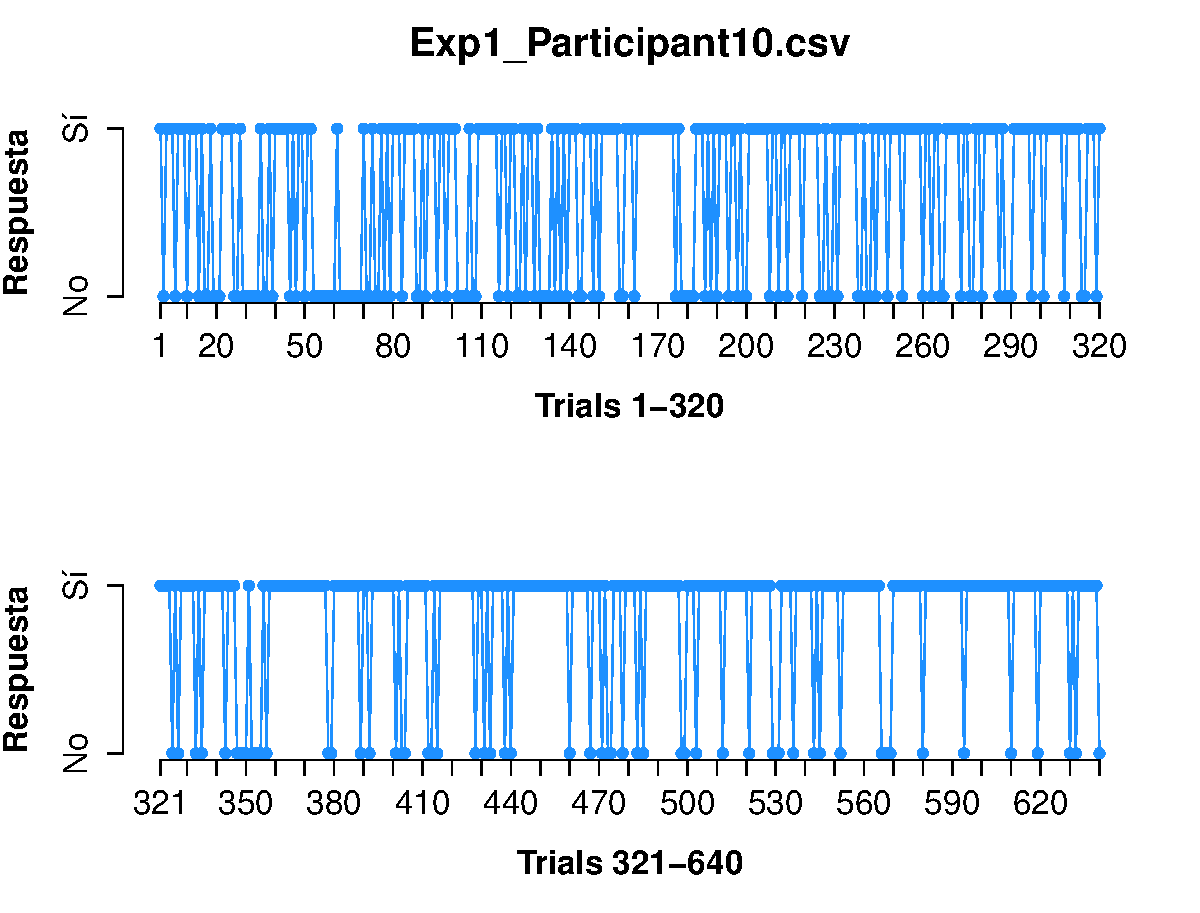
\includegraphics[width=0.30\textwidth]{Figures/Response_Exp1_P10} \includegraphics[width=0.30\textwidth]{Figures/Response_Exp1_P11} \includegraphics[width=0.30\textwidth]{Figures/Response_Exp1_P12}
\includegraphics[width=0.30\textwidth]{Figures/Response_Exp1_P13} \includegraphics[width=0.30\textwidth]{Figures/Response_Exp1_P14} \includegraphics[width=0.30\textwidth]{Figures/Response_Exp1_P15}
\includegraphics[width=0.30\textwidth]{Figures/Response_Exp1_P16} \includegraphics[width=0.30\textwidth]{Figures/Response_Exp1_P17} \includegraphics[width=0.30\textwidth]{Figures/Response_Exp1_P18}
\includegraphics[width=0.30\textwidth]{Figures/Response_Exp1_P19} \includegraphics[width=0.30\textwidth]{Figures/Response_Exp1_P20} \includegraphics[width=0.30\textwidth]{Figures/Response_Exp1_P21} 
%\decoRule
\caption[Response_Exp1]{Respuesta registrada ensayo a ensayo durante la tarea de detección binaria para cada uno de los veintiun participantes en el Experimento 1. Por cada participante, se muestran dos gráficas separadas para una mejor apreciación de sus elecciones durante la primera y segunda mitad del procedimiento.}
\label{fig:Response_E1}
\end{figure}



\begin{figure}[th]
\centering
\includegraphics[width=0.30\textwidth]{Figures/Response_Exp2_P1} \includegraphics[width=0.30\textwidth]{Figures/Response_Exp2_P2} \includegraphics[width=0.30\textwidth]{Figures/Response_Exp2_P3}
\includegraphics[width=0.30\textwidth]{Figures/Response_Exp2_P4} \includegraphics[width=0.30\textwidth]{Figures/Response_Exp2_P5} \includegraphics[width=0.30\textwidth]{Figures/Response_Exp2_P6}
\includegraphics[width=0.30\textwidth]{Figures/Response_Exp2_P7} \includegraphics[width=0.30\textwidth]{Figures/Response_Exp2_P8} \includegraphics[width=0.30\textwidth]{Figures/Response_Exp2_P9}
\includegraphics[width=0.30\textwidth]{Figures/Response_Exp2_P10} \includegraphics[width=0.30\textwidth]{Figures/Response_Exp2_P11} \includegraphics[width=0.30\textwidth]{Figures/Response_Exp2_P12}
\includegraphics[width=0.30\textwidth]{Figures/Response_Exp2_P13} \includegraphics[width=0.30\textwidth]{Figures/Response_Exp2_P14} \includegraphics[width=0.30\textwidth]{Figures/Response_Exp2_P15}
\includegraphics[width=0.30\textwidth]{Figures/Response_Exp2_P16} \includegraphics[width=0.30\textwidth]{Figures/Response_Exp2_P17} \includegraphics[width=0.30\textwidth]{Figures/Response_Exp2_P18}
\includegraphics[width=0.30\textwidth]{Figures/Response_Exp2_P19} \includegraphics[width=0.30\textwidth]{Figures/Response_Exp2_P20} 
%\decoRule
\caption[Response_Exp2]{Respuesta registrada ensayo a ensayo durante la tarea de detección binaria para cada uno de los veinte participantes en el Experimento 2. Por cada participante, se muestran dos gráficas separadas para una mejor apreciación de sus elecciones durante la primera y segunda mitad del procedimiento.}
\label{fig:Response_E2}
\end{figure}


\item Correlación entre las respuestas emitidas 'Sí/No' y el tipo de estímulo presentado en cada ensayo.



\begin{figure}[th]
\centering
\includegraphics[width=0.60\textwidth]{Figures/BiasResp_Exp1_P1} 
%\decoRule
\caption[ParticipanteSesgado_Variables]{,}
\label{fig:BiasResp_E1_P1}
\end{figure}



\begin{figure}[th]
\centering
\includegraphics[width=0.30\textwidth]{Figures/BiasResp_Exp1_P1} \includegraphics[width=0.30\textwidth]{Figures/BiasResp_Exp1_P2} \includegraphics[width=0.30\textwidth]{Figures/BiasResp_Exp1_P3}
\includegraphics[width=0.30\textwidth]{Figures/BiasResp_Exp1_P4} \includegraphics[width=0.30\textwidth]{Figures/BiasResp_Exp1_P5} \includegraphics[width=0.30\textwidth]{Figures/BiasResp_Exp1_P6}
\includegraphics[width=0.30\textwidth]{Figures/BiasResp_Exp1_P7} \includegraphics[width=0.30\textwidth]{Figures/BiasResp_Exp1_P8} \includegraphics[width=0.30\textwidth]{Figures/BiasResp_Exp1_P9}
\includegraphics[width=0.30\textwidth]{Figures/BiasResp_Exp1_P10} \includegraphics[width=0.30\textwidth]{Figures/BiasResp_Exp1_P11} \includegraphics[width=0.30\textwidth]{Figures/BiasResp_Exp1_P12}
\includegraphics[width=0.30\textwidth]{Figures/BiasResp_Exp1_P13} \includegraphics[width=0.30\textwidth]{Figures/BiasResp_Exp1_P14} \includegraphics[width=0.30\textwidth]{Figures/BiasResp_Exp1_P15}
\includegraphics[width=0.30\textwidth]{Figures/BiasResp_Exp1_P16} \includegraphics[width=0.30\textwidth]{Figures/BiasResp_Exp1_P17} \includegraphics[width=0.30\textwidth]{Figures/BiasResp_Exp1_P18}
\includegraphics[width=0.30\textwidth]{Figures/BiasResp_Exp1_P19} \includegraphics[width=0.30\textwidth]{Figures/BiasResp_Exp1_P20} \includegraphics[width=0.30\textwidth]{Figures/BiasResp_Exp1_P21}
%\decoRule
\caption[Sesgo al Responder _Ex1]{Respuesta registrada por cada ensayo durante la tarea de detección binaria por cada uno de los veintiun participantes del Experimento 1. Por cada participante, se muestran tres gráficos distintos que relacionan la respuesta emitida en cada ensayo con la naturaleza del estímulo en cuestión; en el gráfico superior, se señalan con color púrpura los ensayos en que se mostró un estímulo difícil y en azul, los fáciles; en el panel intermedio se muestran en verde los estímulos donde los círculos a comparar eran del mismo tamaño (señal), y en rojo los ensayos en que esto no era el caso (ruido); el panel inferior muestra el color del estímulo en pantalla.}
\label{fig:BiasResp_E1}
\end{figure}



\item Emisión de r

En el caso de la escala de confianza presentada tras el registro del juicio de detección, donde los participantes indicaron qué tan seguros se encontraban de su respuesta, interesa revisar que los participantes estuvieran dedicando suficiente atención a esta segunda tarea lo suficiente como para utilizar todas las opciones de respuesta.  Las Figuras~\ref{fig:Rating_E2} muestran, a lo largo de la tarea, cada uno de los valores de confianza .\\

\begin{figure}[th]
\centering
\includegraphics[width=0.30\textwidth]{Figures/Rating_Exp2_P1} \includegraphics[width=0.30\textwidth]{Figures/Rating_Exp2_P2} \includegraphics[width=0.30\textwidth]{Figures/Rating_Exp2_P3}
\includegraphics[width=0.30\textwidth]{Figures/Rating_Exp2_P4} \includegraphics[width=0.30\textwidth]{Figures/Rating_Exp2_P5} \includegraphics[width=0.30\textwidth]{Figures/Rating_Exp2_P6}
\includegraphics[width=0.30\textwidth]{Figures/Rating_Exp2_P7} \includegraphics[width=0.30\textwidth]{Figures/Rating_Exp2_P8} \includegraphics[width=0.30\textwidth]{Figures/Rating_Exp2_P9}
\includegraphics[width=0.30\textwidth]{Figures/Rating_Exp2_P10} \includegraphics[width=0.30\textwidth]{Figures/Rating_Exp2_P11} \includegraphics[width=0.30\textwidth]{Figures/Rating_Exp2_P12}
\includegraphics[width=0.30\textwidth]{Figures/Rating_Exp2_P13} \includegraphics[width=0.30\textwidth]{Figures/Rating_Exp2_P14} \includegraphics[width=0.30\textwidth]{Figures/Rating_Exp2_P15}
\includegraphics[width=0.30\textwidth]{Figures/Rating_Exp2_P16} \includegraphics[width=0.30\textwidth]{Figures/Rating_Exp2_P17} \includegraphics[width=0.30\textwidth]{Figures/Rating_Exp2_P18}
\includegraphics[width=0.30\textwidth]{Figures/Rating_Exp2_P19} \includegraphics[width=0.30\textwidth]{Figures/Rating_Exp2_P20} 
%\decoRule
\caption[Rating_Exp2]{Respuesta registrada ensayo a ensayo, por cada uno de los veinte participantes del Experimento 2, }
\label{fig:Rating_E2}
\end{figure}

\end{itemize}



\subsection{Control 2: Evaluando tiempos de respuesta a lo largo del experimento}


%%%%%%%%%%%%%%%%%%%%%%%%%%%%%%%%%%%%%%%%%%%%%%%%%%%%%%%%%%%%%%
%%%%%%%%%  Respuesta Rating en los ensayos
% Experimento 2
%%%%%%%%%%%%%%%%%%%%%%%%%%%%%%%%%%%%%%%%%%%%%%%%%%%%%%%%%%%%%%%
\begin{figure}[th]
\centering
\includegraphics[width=0.30\textwidth]{Figures/RTs_Exp2_P1} \includegraphics[width=0.30\textwidth]{Figures/RTs_Exp2_P2} \includegraphics[width=0.30\textwidth]{Figures/RTs_Exp2_P3}
\includegraphics[width=0.30\textwidth]{Figures/RTs_Exp2_P4} \includegraphics[width=0.30\textwidth]{Figures/RTs_Exp2_P5} \includegraphics[width=0.30\textwidth]{Figures/RTs_Exp2_P6}
\includegraphics[width=0.30\textwidth]{Figures/RTs_Exp2_P7} \includegraphics[width=0.30\textwidth]{Figures/RTs_Exp2_P8} \includegraphics[width=0.30\textwidth]{Figures/RTs_Exp2_P9}
\includegraphics[width=0.30\textwidth]{Figures/RTs_Exp2_P10} \includegraphics[width=0.30\textwidth]{Figures/RTs_Exp2_P11} \includegraphics[width=0.30\textwidth]{Figures/RTs_Exp2_P12}
\includegraphics[width=0.30\textwidth]{Figures/RTs_Exp2_P13} \includegraphics[width=0.30\textwidth]{Figures/RTs_Exp2_P14} \includegraphics[width=0.30\textwidth]{Figures/RTs_Exp2_P15}
\includegraphics[width=0.30\textwidth]{Figures/RTs_Exp2_P16} \includegraphics[width=0.30\textwidth]{Figures/RTs_Exp2_P17} \includegraphics[width=0.30\textwidth]{Figures/RTs_Exp2_P18}
\includegraphics[width=0.30\textwidth]{Figures/RTs_Exp2_P19} \includegraphics[width=0.30\textwidth]{Figures/RTs_Exp2_P20} 
%\decoRule
\caption[TRs_Exp2]{Tiempos de Respuesta por ensayo (Experimento 2). Se muestran simultáneamente el tiempo de respuesta a la tarea principal (Color X) y a la escala de confianza (Color Y).}
\label{fig:RTs_E2}
\end{figure}


%%%%%%%%%%%%%%%%%%%%%%%%%%%%%%%%%%%%%%%%%%%%%%%%%%%%%%%%%%%%%%
%%%%%%%%%  Respuesta Rating en los ensayos
% Experimento 2
%%%%%%%%%%%%%%%%%%%%%%%%%%%%%%%%%%%%%%%%%%%%%%%%%%%%%%%%%%%%%%%
\begin{figure}[th]
\centering
\includegraphics[width=0.30\textwidth]{Figures/RT1_Exp2_P1} \includegraphics[width=0.30\textwidth]{Figures/RT1_Exp2_P2} \includegraphics[width=0.30\textwidth]{Figures/RT1_Exp2_P3}
\includegraphics[width=0.30\textwidth]{Figures/RT1_Exp2_P4} \includegraphics[width=0.30\textwidth]{Figures/RT1_Exp2_P5} \includegraphics[width=0.30\textwidth]{Figures/RT1_Exp2_P6}
\includegraphics[width=0.30\textwidth]{Figures/RT1_Exp2_P7} \includegraphics[width=0.30\textwidth]{Figures/RT1_Exp2_P8} \includegraphics[width=0.30\textwidth]{Figures/RT1_Exp2_P9}
\includegraphics[width=0.30\textwidth]{Figures/RT1_Exp2_P10} \includegraphics[width=0.30\textwidth]{Figures/RT1_Exp2_P11} \includegraphics[width=0.30\textwidth]{Figures/RT1_Exp2_P12}
\includegraphics[width=0.30\textwidth]{Figures/RT1_Exp2_P13} \includegraphics[width=0.30\textwidth]{Figures/RT1_Exp2_P14} \includegraphics[width=0.30\textwidth]{Figures/RT1_Exp2_P15}
\includegraphics[width=0.30\textwidth]{Figures/RT1_Exp2_P16} \includegraphics[width=0.30\textwidth]{Figures/RT1_Exp2_P17} \includegraphics[width=0.30\textwidth]{Figures/RT1_Exp2_P18}
\includegraphics[width=0.30\textwidth]{Figures/RT1_Exp2_P19} \includegraphics[width=0.30\textwidth]{Figures/RT1_Exp2_P20} 
%\decoRule
\caption[TR1_Exp2]{Tiempo de Respuesta a la tarea perceptual por ensayo (Experimento 2).}
\label{fig:RT1_E2}
\end{figure}


%%%%%%%%%%%%%%%%%%%%%%%%%%%%%%%%%%%%%%%%%%%%%%%%%%%%%%%%%%%%%%
%%%%%%%%%  Respuesta Rating en los ensayos
% Experimento 2
%%%%%%%%%%%%%%%%%%%%%%%%%%%%%%%%%%%%%%%%%%%%%%%%%%%%%%%%%%%%%%%
\begin{figure}[th]
\centering
\includegraphics[width=0.30\textwidth]{Figures/RT2_Exp2_P1} \includegraphics[width=0.30\textwidth]{Figures/RT2_Exp2_P2} \includegraphics[width=0.30\textwidth]{Figures/RT2_Exp2_P3}
\includegraphics[width=0.30\textwidth]{Figures/RT2_Exp2_P4} \includegraphics[width=0.30\textwidth]{Figures/RT2_Exp2_P5} \includegraphics[width=0.30\textwidth]{Figures/RT2_Exp2_P6}
\includegraphics[width=0.30\textwidth]{Figures/RT2_Exp2_P7} \includegraphics[width=0.30\textwidth]{Figures/RT2_Exp2_P8} \includegraphics[width=0.30\textwidth]{Figures/RT2_Exp2_P9}
\includegraphics[width=0.30\textwidth]{Figures/RT2_Exp2_P10} \includegraphics[width=0.30\textwidth]{Figures/RT2_Exp2_P11} \includegraphics[width=0.30\textwidth]{Figures/RT2_Exp2_P12}
\includegraphics[width=0.30\textwidth]{Figures/RT2_Exp2_P13} \includegraphics[width=0.30\textwidth]{Figures/RT2_Exp2_P14} \includegraphics[width=0.30\textwidth]{Figures/RT2_Exp2_P15}
\includegraphics[width=0.30\textwidth]{Figures/RT2_Exp2_P16} \includegraphics[width=0.30\textwidth]{Figures/RT2_Exp2_P17} \includegraphics[width=0.30\textwidth]{Figures/RT2_Exp2_P18}
\includegraphics[width=0.30\textwidth]{Figures/RT2_Exp2_P19} \includegraphics[width=0.30\textwidth]{Figures/RT2_Exp2_P20} 
%\decoRule
\caption[TR2_Exp2]{Tiempo de respuesta a la escala de confianza por ensayo (Experimento 2).}
\label{fig:RT2_E2}
\end{figure}



\subsection{Control 3: ¿La duración del experimento tuvo un impacto en la ejecución de los participantes?}


%%%%%%%%%%%%%%%%%%%%%%%%%%%%%%%%%%%%%%%%%%%%%%%%%%%%%%%%%%%%%%
%%%%%%%%%  Respuesta (Y/N) en los ensayos
% Experimento 2
%%%%%%%%%%%%%%%%%%%%%%%%%%%%%%%%%%%%%%%%%%%%%%%%%%%%%%%%%%%%%%%
\begin{figure}[th]
\centering
\includegraphics[width=0.30\textwidth]{Figures/Success_Exp1_P1} \includegraphics[width=0.30\textwidth]{Figures/Success_Exp1_P2} \includegraphics[width=0.30\textwidth]{Figures/Success_Exp1_P3}
\includegraphics[width=0.30\textwidth]{Figures/Success_Exp1_P4} \includegraphics[width=0.30\textwidth]{Figures/Success_Exp1_P5} \includegraphics[width=0.30\textwidth]{Figures/Success_Exp1_P6}
\includegraphics[width=0.30\textwidth]{Figures/Success_Exp1_P7} \includegraphics[width=0.30\textwidth]{Figures/Success_Exp1_P8} \includegraphics[width=0.30\textwidth]{Figures/Success_Exp1_P9}
\includegraphics[width=0.30\textwidth]{Figures/Success_Exp1_P10} \includegraphics[width=0.30\textwidth]{Figures/Success_Exp1_P11} \includegraphics[width=0.30\textwidth]{Figures/Success_Exp1_P12}
\includegraphics[width=0.30\textwidth]{Figures/Success_Exp1_P13} \includegraphics[width=0.30\textwidth]{Figures/Success_Exp1_P14} \includegraphics[width=0.30\textwidth]{Figures/Success_Exp1_P15}
\includegraphics[width=0.30\textwidth]{Figures/Success_Exp1_P16} \includegraphics[width=0.30\textwidth]{Figures/Success_Exp1_P17} \includegraphics[width=0.30\textwidth]{Figures/Success_Exp1_P18}
\includegraphics[width=0.30\textwidth]{Figures/Success_Exp1_P19} \includegraphics[width=0.30\textwidth]{Figures/Success_Exp1_P20} \includegraphics[width=0.30\textwidth]{Figures/Success_Exp1_P21} 
%\decoRule
\caption[Success_Exp1]{Desempeño del participante a lo largo del experimento (Experimento 1).}
\label{fig:Success_E1}
\end{figure}


\begin{figure}[th]
\centering
\includegraphics[width=0.30\textwidth]{Figures/Success_Exp2_P1} \includegraphics[width=0.30\textwidth]{Figures/Success_Exp2_P2} \includegraphics[width=0.30\textwidth]{Figures/Success_Exp2_P3}
\includegraphics[width=0.30\textwidth]{Figures/Success_Exp2_P4} \includegraphics[width=0.30\textwidth]{Figures/Success_Exp2_P5} \includegraphics[width=0.30\textwidth]{Figures/Success_Exp2_P6}
\includegraphics[width=0.30\textwidth]{Figures/Success_Exp2_P7} \includegraphics[width=0.30\textwidth]{Figures/Success_Exp2_P8} \includegraphics[width=0.30\textwidth]{Figures/Success_Exp2_P9}
\includegraphics[width=0.30\textwidth]{Figures/Success_Exp2_P10} \includegraphics[width=0.30\textwidth]{Figures/Success_Exp2_P11} \includegraphics[width=0.30\textwidth]{Figures/Success_Exp2_P12}
\includegraphics[width=0.30\textwidth]{Figures/Success_Exp2_P13} \includegraphics[width=0.30\textwidth]{Figures/Success_Exp2_P14} \includegraphics[width=0.30\textwidth]{Figures/Success_Exp2_P15}
\includegraphics[width=0.30\textwidth]{Figures/Success_Exp2_P16} \includegraphics[width=0.30\textwidth]{Figures/Success_Exp2_P17} \includegraphics[width=0.30\textwidth]{Figures/Success_Exp2_P18}
\includegraphics[width=0.30\textwidth]{Figures/Success_Exp2_P19} \includegraphics[width=0.30\textwidth]{Figures/Success_Exp2_P20} 
%\decoRule
\caption[Success_Exp2]{Desempeño del participante a lo largo del experimento (Experimento 2).}
\label{fig:Success_E2}
\end{figure}


%%%%%%%%%%%%%%%%%%%%%%%%%%%%%%%%%%%%%%%%%%%%%%%%%%%%%%%%
%%%%%%%%%  Respuesta Rating en los ensayos
% Experimento 2
%%%%%%%%%%%%%%%%%%%%%%%%%%%%%%%%%%%%%%%%%%%%%%%%%%%%%%%%%%%%%%%
\begin{figure}[th]
\centering
\includegraphics[width=0.30\textwidth]{Figures/Outcome_Exp1_P1} \includegraphics[width=0.30\textwidth]{Figures/Outcome_Exp1_P2} \includegraphics[width=0.30\textwidth]{Figures/Outcome_Exp1_P3}
\includegraphics[width=0.30\textwidth]{Figures/Outcome_Exp1_P4} \includegraphics[width=0.30\textwidth]{Figures/Outcome_Exp1_P5} \includegraphics[width=0.30\textwidth]{Figures/Outcome_Exp1_P6}
\includegraphics[width=0.30\textwidth]{Figures/Outcome_Exp1_P7} \includegraphics[width=0.30\textwidth]{Figures/Outcome_Exp1_P8} \includegraphics[width=0.30\textwidth]{Figures/Outcome_Exp1_P9}
\includegraphics[width=0.30\textwidth]{Figures/Outcome_Exp1_P10} \includegraphics[width=0.30\textwidth]{Figures/Outcome_Exp1_P11} \includegraphics[width=0.30\textwidth]{Figures/Outcome_Exp1_P12}
\includegraphics[width=0.30\textwidth]{Figures/Outcome_Exp1_P13} \includegraphics[width=0.30\textwidth]{Figures/Outcome_Exp1_P14} \includegraphics[width=0.30\textwidth]{Figures/Outcome_Exp1_P15}
\includegraphics[width=0.30\textwidth]{Figures/Outcome_Exp1_P16} \includegraphics[width=0.30\textwidth]{Figures/Outcome_Exp1_P17} \includegraphics[width=0.30\textwidth]{Figures/Outcome_Exp1_P18}
\includegraphics[width=0.30\textwidth]{Figures/Outcome_Exp1_P19} \includegraphics[width=0.30\textwidth]{Figures/Outcome_Exp1_P20} \includegraphics[width=0.30\textwidth]{Figures/Outcome_Exp1_P21} 
%\decoRule
\caption[Outcome_Exp1]{Resultado obtenido por ensayo (discerniendo entre tipos de acierto y errores) (Experimento 1).}
\label{fig:Outcome_E1}
\end{figure}



\begin{figure}[th]
\centering
\includegraphics[width=0.30\textwidth]{Figures/Outcome_Exp2_P1} \includegraphics[width=0.30\textwidth]{Figures/Outcome_Exp2_P2} \includegraphics[width=0.30\textwidth]{Figures/Outcome_Exp2_P3}
\includegraphics[width=0.30\textwidth]{Figures/Outcome_Exp2_P4} \includegraphics[width=0.30\textwidth]{Figures/Outcome_Exp2_P5} \includegraphics[width=0.30\textwidth]{Figures/Outcome_Exp2_P6}
\includegraphics[width=0.30\textwidth]{Figures/Outcome_Exp2_P7} \includegraphics[width=0.30\textwidth]{Figures/Outcome_Exp2_P8} \includegraphics[width=0.30\textwidth]{Figures/Outcome_Exp2_P9}
\includegraphics[width=0.30\textwidth]{Figures/Outcome_Exp2_P10} \includegraphics[width=0.30\textwidth]{Figures/Outcome_Exp2_P11} \includegraphics[width=0.30\textwidth]{Figures/Outcome_Exp2_P12}
\includegraphics[width=0.30\textwidth]{Figures/Outcome_Exp2_P13} \includegraphics[width=0.30\textwidth]{Figures/Outcome_Exp2_P14} \includegraphics[width=0.30\textwidth]{Figures/Outcome_Exp2_P15}
\includegraphics[width=0.30\textwidth]{Figures/Outcome_Exp2_P16} \includegraphics[width=0.30\textwidth]{Figures/Outcome_Exp2_P17} \includegraphics[width=0.30\textwidth]{Figures/Outcome_Exp2_P18}
\includegraphics[width=0.30\textwidth]{Figures/Outcome_Exp2_P19} \includegraphics[width=0.30\textwidth]{Figures/Outcome_Exp2_P20} 
%\decoRule
\caption[Outcome_Exp2]{Resultado obtenido por cada ensayo (Discerniendo entre tipos de aciertos y errores) (Experimento 2).}
\label{fig:Outcome_E2}
\end{figure}



\subsection{Control 4: ¿Las variables mezcladas para construir los estímulos están afectando el desempeño de los participantes?}



%%%%%%%%%%%%%%%%%%%%%%%%%%%%%%%%%%%%%%%%%%%%%%%%%%%%%%%%%%%%%%
%%%%%%%%%  Efecto Color
% Experimento 2
%%%%%%%%%%%%%%%%%%%%%%%%%%%%%%%%%%%%%%%%%%%%%%%%%%%%%%%%%%%%%%%
\begin{figure}[th]
\centering
\includegraphics[width=0.30\textwidth]{Figures/Color_Exp2_P1} \includegraphics[width=0.30\textwidth]{Figures/Color_Exp2_P2} \includegraphics[width=0.30\textwidth]{Figures/Color_Exp2_P3}
\includegraphics[width=0.30\textwidth]{Figures/Color_Exp2_P4} \includegraphics[width=0.30\textwidth]{Figures/Color_Exp2_P5} \includegraphics[width=0.30\textwidth]{Figures/Color_Exp2_P6}
\includegraphics[width=0.30\textwidth]{Figures/Color_Exp2_P7} \includegraphics[width=0.30\textwidth]{Figures/Color_Exp2_P8} \includegraphics[width=0.30\textwidth]{Figures/Color_Exp2_P9}
\includegraphics[width=0.30\textwidth]{Figures/Color_Exp2_P10} \includegraphics[width=0.30\textwidth]{Figures/Color_Exp2_P11} \includegraphics[width=0.30\textwidth]{Figures/Color_Exp2_P12}
\includegraphics[width=0.30\textwidth]{Figures/Color_Exp2_P13} \includegraphics[width=0.30\textwidth]{Figures/Color_Exp2_P14} \includegraphics[width=0.30\textwidth]{Figures/Color_Exp2_P15}
\includegraphics[width=0.30\textwidth]{Figures/Color_Exp2_P16} \includegraphics[width=0.30\textwidth]{Figures/Color_Exp2_P17} \includegraphics[width=0.30\textwidth]{Figures/Color_Exp2_P18}
\includegraphics[width=0.30\textwidth]{Figures/Color_Exp2_P19} \includegraphics[width=0.30\textwidth]{Figures/Color_Exp2_P20} 
%\decoRule
\caption[Color_Exp2]{Explorando posibles efectos del color de los estímulos (Experimento 2).}
\label{fig:Color_E2}
\end{figure}





%%%%%%%%%%%%%%%%%%%%%%%%%%%%%%%%%%%%%%%%%%%%%%%%%%%%%%%%%%%%%%
%%%%%%%%%  Efecto Numero Circulos Externos
% Experimento 2
%%%%%%%%%%%%%%%%%%%%%%%%%%%%%%%%%%%%%%%%%%%%%%%%%%%%%%%%%%%%%%%
\begin{figure}[th]
\centering
\includegraphics[width=0.30\textwidth]{Figures/Numero_Exp2_P1} \includegraphics[width=0.30\textwidth]{Figures/Numero_Exp2_P2} \includegraphics[width=0.30\textwidth]{Figures/Numero_Exp2_P3}
\includegraphics[width=0.30\textwidth]{Figures/Numero_Exp2_P4} \includegraphics[width=0.30\textwidth]{Figures/Numero_Exp2_P5} \includegraphics[width=0.30\textwidth]{Figures/Numero_Exp2_P6}
\includegraphics[width=0.30\textwidth]{Figures/Numero_Exp2_P7} \includegraphics[width=0.30\textwidth]{Figures/Numero_Exp2_P8} \includegraphics[width=0.30\textwidth]{Figures/Numero_Exp2_P9}
\includegraphics[width=0.30\textwidth]{Figures/Numero_Exp2_P10} \includegraphics[width=0.30\textwidth]{Figures/Numero_Exp2_P11} \includegraphics[width=0.30\textwidth]{Figures/Numero_Exp2_P12}
\includegraphics[width=0.30\textwidth]{Figures/Numero_Exp2_P13} \includegraphics[width=0.30\textwidth]{Figures/Numero_Exp2_P14} \includegraphics[width=0.30\textwidth]{Figures/Numero_Exp2_P15}
\includegraphics[width=0.30\textwidth]{Figures/Numero_Exp2_P16} \includegraphics[width=0.30\textwidth]{Figures/Numero_Exp2_P17} \includegraphics[width=0.30\textwidth]{Figures/Numero_Exp2_P18}
\includegraphics[width=0.30\textwidth]{Figures/Numero_Exp2_P19} \includegraphics[width=0.30\textwidth]{Figures/Numero_Exp2_P20} 
%\decoRule
\caption[Numero_Exp2]{Efecto del Numero de Circulos Externos (Experimento 2).}
\label{fig:Numero_E2}
\end{figure}


----------------------------------------------------------------------------------------
%	SECTION 2
%----------------------------------------------------------------------------------------

\section{Evidencia del Efecto Espejo}

%%%%%%%%%%%%%%%%%%%%%%%%%%%%%%%%%%%%%%%%%%%%%%%%%%%%%%%%%%%%%%
%%%%%%%%%  Mirror Effect
% Experimento 2
%%%%%%%%%%%%%%%%%%%%%%%%%%%%%%%%%%%%%%%%%%%%%%%%%%%%%%%%%%%%%%%

\begin{figure}[th]
\centering
\includegraphics[width=0.30\textwidth]{Figures/MirrorRate_Exp1_P1} \includegraphics[width=0.30\textwidth]{Figures/MirrorRate_Exp1_P2} \includegraphics[width=0.30\textwidth]{Figures/MirrorRate_Exp1_P3}
\includegraphics[width=0.30\textwidth]{Figures/MirrorRate_Exp1_P4} \includegraphics[width=0.30\textwidth]{Figures/MirrorRate_Exp1_P5} \includegraphics[width=0.30\textwidth]{Figures/MirrorRate_Exp1_P6}
\includegraphics[width=0.30\textwidth]{Figures/MirrorRate_Exp1_P7} \includegraphics[width=0.30\textwidth]{Figures/MirrorRate_Exp1_P8} \includegraphics[width=0.30\textwidth]{Figures/MirrorRate_Exp1_P9}
\includegraphics[width=0.30\textwidth]{Figures/MirrorRate_Exp1_P10} \includegraphics[width=0.30\textwidth]{Figures/MirrorRate_Exp1_P11} \includegraphics[width=0.30\textwidth]{Figures/MirrorRate_Exp1_P12}
\includegraphics[width=0.30\textwidth]{Figures/MirrorRate_Exp1_P13} \includegraphics[width=0.30\textwidth]{Figures/MirrorRate_Exp1_P14} \includegraphics[width=0.30\textwidth]{Figures/MirrorRate_Exp1_P15}
\includegraphics[width=0.30\textwidth]{Figures/MirrorRate_Exp1_P16} \includegraphics[width=0.30\textwidth]{Figures/MirrorRate_Exp1_P17} \includegraphics[width=0.30\textwidth]{Figures/MirrorRate_Exp1_P18}
\includegraphics[width=0.30\textwidth]{Figures/MirrorRate_Exp1_P19} \includegraphics[width=0.30\textwidth]{Figures/MirrorRate_Exp1_P20} \includegraphics[width=0.30\textwidth]{Figures/MirrorRate_Exp1_P21} 
%\decoRule
\caption[Rate_Exp1]{Evaluando el patrón de Hits y Falsas Alarmas identificado como Efecto Espejo (Experimento 1)}
\label{fig:Rate_E1}
\end{figure}


\begin{figure}[th]
\centering
\includegraphics[width=0.30\textwidth]{Figures/MirrorRate_Exp2_P1} \includegraphics[width=0.30\textwidth]{Figures/MirrorRate_Exp2_P2} \includegraphics[width=0.30\textwidth]{Figures/MirrorRate_Exp2_P3}
\includegraphics[width=0.30\textwidth]{Figures/MirrorRate_Exp2_P4} \includegraphics[width=0.30\textwidth]{Figures/MirrorRate_Exp2_P5} \includegraphics[width=0.30\textwidth]{Figures/MirrorRate_Exp2_P6}
\includegraphics[width=0.30\textwidth]{Figures/MirrorRate_Exp2_P7} \includegraphics[width=0.30\textwidth]{Figures/MirrorRate_Exp2_P8} \includegraphics[width=0.30\textwidth]{Figures/MirrorRate_Exp2_P9}
\includegraphics[width=0.30\textwidth]{Figures/MirrorRate_Exp2_P10} \includegraphics[width=0.30\textwidth]{Figures/MirrorRate_Exp2_P11} \includegraphics[width=0.30\textwidth]{Figures/MirrorRate_Exp2_P12}
\includegraphics[width=0.30\textwidth]{Figures/MirrorRate_Exp2_P13} \includegraphics[width=0.30\textwidth]{Figures/MirrorRate_Exp2_P14} \includegraphics[width=0.30\textwidth]{Figures/MirrorRate_Exp2_P15}
\includegraphics[width=0.30\textwidth]{Figures/MirrorRate_Exp2_P16} \includegraphics[width=0.30\textwidth]{Figures/MirrorRate_Exp2_P17} \includegraphics[width=0.30\textwidth]{Figures/MirrorRate_Exp2_P18}
\includegraphics[width=0.30\textwidth]{Figures/MirrorRate_Exp2_P19} \includegraphics[width=0.30\textwidth]{Figures/MirrorRate_Exp2_P20} 
%\decoRule
\caption[Rate_Exp2]{Evaluando el patrón de Hits y Falsas Alarmas identificado como Efecto Espejo (Experimento 2)}
\label{fig:Rate_E2}
\end{figure}





%%%%%%%%%%%%%%%%%%%%%%%%%%%%%%%%%%%%%%%%%%%%%%%%%%%%%%%%%%%%%%
%%%%%%%%%  Mirror Effect - Confidence Rating
% Experimento 2
%%%%%%%%%%%%%%%%%%%%%%%%%%%%%%%%%%%%%%%%%%%%%%%%%%%%%%%%%%%%%%%

\begin{figure}[th]
\centering
\includegraphics[width=0.30\textwidth]{Figures/MirrorRating_Exp1_P1} \includegraphics[width=0.30\textwidth]{Figures/MirrorRating_Exp1_P2} \includegraphics[width=0.30\textwidth]{Figures/MirrorRating_Exp1_P3}
\includegraphics[width=0.30\textwidth]{Figures/MirrorRating_Exp1_P4} \includegraphics[width=0.30\textwidth]{Figures/MirrorRating_Exp1_P5} \includegraphics[width=0.30\textwidth]{Figures/MirrorRating_Exp1_P6}
\includegraphics[width=0.30\textwidth]{Figures/MirrorRating_Exp1_P7} \includegraphics[width=0.30\textwidth]{Figures/MirrorRating_Exp1_P8} \includegraphics[width=0.30\textwidth]{Figures/MirrorRating_Exp1_P9}
\includegraphics[width=0.30\textwidth]{Figures/MirrorRating_Exp1_P10} \includegraphics[width=0.30\textwidth]{Figures/MirrorRating_Exp1_P11} \includegraphics[width=0.30\textwidth]{Figures/MirrorRating_Exp1_P12}
\includegraphics[width=0.30\textwidth]{Figures/MirrorRating_Exp1_P13} \includegraphics[width=0.30\textwidth]{Figures/MirrorRating_Exp1_P14} \includegraphics[width=0.30\textwidth]{Figures/MirrorRating_Exp1_P15}
\includegraphics[width=0.30\textwidth]{Figures/MirrorRating_Exp1_P16} \includegraphics[width=0.30\textwidth]{Figures/MirrorRating_Exp1_P17} \includegraphics[width=0.30\textwidth]{Figures/MirrorRating_Exp1_P18}
\includegraphics[width=0.30\textwidth]{Figures/MirrorRating_Exp1_P19} \includegraphics[width=0.30\textwidth]{Figures/MirrorRating_Exp1_P20} \includegraphics[width=0.30\textwidth]{Figures/MirrorRating_Exp1_P21} 
%\decoRule
\caption[MErating_Ex1]{Evaluando el patrón de puntajes de confianza asignados (Experimento 1)}
\label{fig:MERating_E1}
\end{figure}



\begin{figure}[th]
\centering
\includegraphics[width=0.30\textwidth]{Figures/MirrorRating_Exp2_P1} \includegraphics[width=0.30\textwidth]{Figures/MirrorRating_Exp2_P2} \includegraphics[width=0.30\textwidth]{Figures/MirrorRating_Exp2_P3}
\includegraphics[width=0.30\textwidth]{Figures/MirrorRating_Exp2_P4} \includegraphics[width=0.30\textwidth]{Figures/MirrorRating_Exp2_P5} \includegraphics[width=0.30\textwidth]{Figures/MirrorRating_Exp2_P6}
\includegraphics[width=0.30\textwidth]{Figures/MirrorRating_Exp2_P7} \includegraphics[width=0.30\textwidth]{Figures/MirrorRating_Exp2_P8} \includegraphics[width=0.30\textwidth]{Figures/MirrorRating_Exp2_P9}
\includegraphics[width=0.30\textwidth]{Figures/MirrorRating_Exp2_P10} \includegraphics[width=0.30\textwidth]{Figures/MirrorRating_Exp2_P11} \includegraphics[width=0.30\textwidth]{Figures/MirrorRating_Exp2_P12}
\includegraphics[width=0.30\textwidth]{Figures/MirrorRating_Exp2_P13} \includegraphics[width=0.30\textwidth]{Figures/MirrorRating_Exp2_P14} \includegraphics[width=0.30\textwidth]{Figures/MirrorRating_Exp2_P15}
\includegraphics[width=0.30\textwidth]{Figures/MirrorRating_Exp2_P16} \includegraphics[width=0.30\textwidth]{Figures/MirrorRating_Exp2_P17} \includegraphics[width=0.30\textwidth]{Figures/MirrorRating_Exp2_P18}
\includegraphics[width=0.30\textwidth]{Figures/MirrorRating_Exp2_P19} \includegraphics[width=0.30\textwidth]{Figures/MirrorRating_Exp2_P20} 
%\decoRule
\caption[MERating_Exp2]{Evaluando el patrón de puntajes de confianza identificados como Efecto Espejo (Experimento 2)}
\label{fig:MERating_E2}
\end{figure}












%Oara ACA (2017-2)
 
-Introduccion (Cosas que bajar, blablabla) - Clase de Como bajar/correr todo
-Pre-Requisitos: Parte Matematica
-------Introduccion a Modelos Bayesianos (Teorema de Bayes; Modelamiento Bayesiano)
------Psicofisica (Funciones ilustrativas)
------Comienzan temas:

1.- Reflejo - Activacion ante estimulo (Killeen)
-Evolucion  y adaptcion (Filosofia de la Ciencia)
2.- Consecuencias - Amibas que siguen estimulacion (Modelo de amibas - Modelo de adaptacion)
3.- Modelos de Aprendizaje (Integrador, RW)
---HallPierce, etc
---Reinforcement LEarning
4.- Psicofísica
5.- Igualacion
6.- Timing

%5532 1222
